% !TeX root = ../thuthesis-example.tex

\chapter{ProSmith Analysis}
\label{chap:2}

\section{Introduction}

In this chapter, we will deep dive into ProSmith, the state-of-the-art model for Michaelis constant
prediction. We will examine the results in more details and see the limitations of the model. The later
chapters will aim to fix these issues and our results and analysis will be further discussed in 
Chapter \ref{chap:6}.

ProSmith offers the best results in terms of MSE and coefficient of determination $r^2$. However, 
these two general metrics fail to see in detail where the model perfoms well and does not. An
alternative to this is to use a hot/cold framework; hot meaning in the training set, and cold 
meaning not in the training set. As the models take two inputs: the protein sequence and 
the substrate string, we can evaluate our metrics for these 4 subgroups: hot proteins and hot substrates, 
hot proteins and cold substrates, cold proteins and hot substrates, and cold proteins and cold substrates. 
This will help evaluate the results, especially for real world applications, as the general metrics fail to help us understand the capabilities of a model in the field of drug design.

Hot proteins and hot substrates means that both the proteins and the substrates are in the training set. It would be useful to adapting existing drugs to new problems. Hot proteins and cold substrates indicates that the proteins are in the training set but the substrates are not. This could improve the research on the use of new chemical compounds on existing enzymes. Cold proteins and hot substrates means that the proteins are not in the training set but that the substrates are. This may be informative to see if current drugs could be use on new enzymes. Finally, the most interesting and promising of all is the cold proteins and cold substrates. Indeed, this could help identify new drugs on new enzymes, which would be completely de novo drug and enzyme design. Furthermore, this will help interpret the generalization of our models. As there are no existing examples in the dataset, the model has to really learn the interactions between the protein and the substrate and cannot simply use its current knownledge to overfit the data and predict results based on the distribution of its inputs.

We expect that the best results will be obtained for the hot proteins and hot substrates subgroup, 
as both the proteins and the substrates are within the training set. This would mean that 
the model leverages its learned patterns and interactions most effectively. 
This scenario is most conducive to the model accurately predicting outcomes based on its training.

On the other hand, the worst results are anticipated for the cold proteins and cold substrates subgroup. 
This is because neither the proteins nor the substrates have been seen by the model during training, 
presenting the most significant challenge in terms of generalization. The model must rely entirely 
on the underlying principles it has learned, without direct knowledge of these specific inputs, 
making accurate prediction considerably more difficult.

For hot proteins and cold substrates, and cold proteins and hot substrates, we expect the results to be in between as we only have half of the information in the training set. We also expect hot proteins and cold substrates to have better results than cold proteins and hot substrates. This is because enzymes are extremely specific and proteins are larger molecules than substrates. Hence, they are more complex and it should be harder for the model to process. 

We replicated ProSmith and obtain a general MSE of 0.604 and a coefficient of determination $r^2$ of 0.563, as well as the same output as the paper offers in their codebase, indicating a successful replication. Using our hot and cold framework, Table \ref{tab:prosmith_results} compiled the results obtained.

\begin{table}[ht]
  \centering
  \begin{tabular}{lcccccc}
  \hline
   & \multicolumn{3}{c}{\textbf{Hot substrate}} & \multicolumn{3}{c}{\textbf{Cold substrate}} \\
   & Samples & MSE & R\(^2\) & Samples & MSE & R\(^2\) \\ \hline
  \textbf{Hot protein}  & 1192 & 0.534 & 0.572 & 64 & 0.678 & 0.545 \\
  \textbf{Cold protein} & 985 & 0.635 & 0.584 & 98 & 1.143 & 0.082 \\ \hline
  \end{tabular}
  \caption{ProSmith results on the test set}
  \label{tab:prosmith_results}
\end{table}

As we observe, while the general results with MSE of 0.604 and coefficient of determination of 0.563, the cold proteins and cold substrates show very dissapointing results and showcase a fault in ProSmith to predict the interactions between completely unseen proteins and substrates in the training set.

More specifically, we see that when both the enzyme and substrate are in the training set (hot proteins and hot substrates), we have better results than the general results, which make sense as we explained above because the model can leverage its learned patterns and interactions most efficiently. What is more surprising however is that we obtain the highest results for the hot substrates and cold proteins, which would mean that the substrate information is more important than the protein's. This raises questions as enzymes are extremely specific and it should be more difficult to predict this value than its counterpart hot protein and cold substrate, as the same enzyme usually works in a similar way and affinity with the substrate may be determined by substrate similarity.

We also obtain decent results for hot proteins and cold substrates, meaning that even though we don't have the information about the substrate in the training set, the model is capable of using its knowledge of proteins and substrates efficiently. However, for cold proteins and cold substrates, the model performs extremely poorly, meaning that it is not capable of generalizing for completely unseen pairs. This becomes very problematic as this would be one of the most important point of the model. Furthermore, it makes us question the model ability to predict the interactions between the protein and the substrate as we get very decent results when some data is in the training set but poor performance when it is not.

This first analysis shed lights on the difficulties of ProSmith to generalize for completely unseen samples and question its overall abilities to predict the interaction between the protein and the substrate and to simply overfit the data.

Hence, in the future, we will not only look at the general metrics of our models but also at these 4
additional metrics that are much more informative.

For our new curated test set, we obtain an MSE of 0.939 and a correlation coefffient $r^2$ of 0.467, as well as the hot/cold results of Table \ref{tab:prosmith_results_new}.

\begin{table}[ht]
  \centering
  \begin{tabular}{lcccccc}
  \hline
   & \multicolumn{3}{c}{\textbf{Hot substrate}} & \multicolumn{3}{c}{\textbf{Cold substrate}} \\
   & Samples & MSE & R\(^2\) & Samples & MSE & R\(^2\) \\ \hline
  \textbf{Hot protein}  & 40 & 0.839 & 0.438 & 30 & 0.731 & -0.140 \\
  \textbf{Cold protein} & 1117 & 0.865 & 0.489 & 102 & 1.833 & 0.108 \\ \hline
  \end{tabular}
  \caption{ProSmith results on the new test set}
  \label{tab:prosmith_results_new}
\end{table}

For the hot proteins and substrates we obtain a coefficient of determination $r^2$ of 0.438, which is inferior to the general value of 0.467. While there are not many samples in this group, only 40, we would expect to have the higher results as the inputs are all in the training set, even though it is for different protein-substrate pairs. 

For the cold proteins and hot substrates, we here have the highest results with a coefficient of determination of 0.489, which is higher than the general value. This is very surprising as this mean that even though we don't have any information about the substrate in the training, the substrate information is enough to predict the Michaelis constant. Considering the very specificity of enzymes, it appears surprising to have higher results when the protein is unknown compared to when it is known, and this deserve further invastigation.

For the hot proteins and cold substrates however, while the MSE is the lowest of all groups, 0.731, the coefficient of determination is negative indicating that the model's predictions inversely correlate with the actual values. This unusual result suggests that while the model can sometimes predict lower errors in terms of MSE, it systematically mispredicts the direction of change in the Michaelis constant when faced with novel substrates paired with known proteins. Essentially, the model might predict higher or lower constants in scenarios where the opposite is true, reflecting a misunderstanding of the underlying biochemical principles or a misalignment between the model's learned patterns and real-world enzymatic behavior. This comment must however been taken with a grain of salt as only 30 samples are available for comparison. Further investigation will be needed to conclude on these results. 

Finally, the cold proteins and substrates shows the worst MSE, 1.833, more than 200\% the values of the other groups, underscoring the inability of the model to generalize and offer decent predictions for completely unseen proteins and substrates. This significant increase in MSE highlights the challenges inherent in extending predictive capabilities to entirely novel enzymatic interactions. The model's performance in this context suggests a critical gap in its learning architecture or training data, which fails to encapsulate the full diversity and complexity of potential enzyme-substrate pairings.

Overall, except for the results of the hot proteins and cold substrates, which have very few samples, we observe a similar trend for the results between the regular test set and the new test set. This indicates that the model is consistent across datasets and hence more reliable that if we had different trends across different dataset. However, we have quite a significant drop between the test set and the new test set, from 0.563 to 0.467, which once again raises the question of the model ability to generalize properly. In the light of these results, it became evident that further investigation was necessary to determine if the model is actually capable of capturing the interactions between the protein and the substrate through the Michaelis constant. To do so, we conducted two experiements. The first one, the single amino acid mutation effect analysis, aims at determining the ability of the model to deal with different but very similar proteins. The second experiment's goal is to see where the Michaelis constant distribution lies between different substrates.

\subsection{Single Amino Acid Mutation Effect Analysis}

Our first experiment is the single amino acid mutation effect. This experiment aims to see how the model
performs when we slightly modify the protein sequence. We focus on a systematic approach where each amino acid in a given protein sequence is individually substituted with one of the other 19 standard amino acids. For instance, consider a protein sequence composed of 500 amino acids. By mutating each position to any of the 19 possible alternatives (excluding the original amino acid at that position), we generate a total of  $500\times19=9,500$ new sequences.

Considering the large number of sequences this would create, we selected 16 sequences of the test set with
8 having a very low MSE, 8 having a very high MSE, and for each of them, 2 hot proteins and hot substrates, 
2 hot proteins and cold substrates, 2 cold proteins and hot substrates, and finally 2 cold proteins and
cold substrates. This allows us to have enough different sequences to make a decent analysis and be
able to compare how it affects the results. 

Once we selected our 16 sequences and created all their mutants, we associated them with the substrate they
originally were with in the test set, hence forming sequence-substrate pairs that can be used by the ProSmith
model and can efficiently be compared to the original sequence-substrate pair.

Below we showcase these results for 2 specific proteins: 
\begin{itemize}
    \item Sequence 1860 which comes from a protein-substrate
    pair where the sequence is not in the training set (cold protein) and the substrate is in the training set 
    (hot substrate) and where the MSE is very low, meaning the Michaelis constant was well predicted.
    \item Sequence 1866 which comes from a protein-substrate pair where the sequence is not in the training set
    (cold protein) and the substrate is in the training set (hot substrate) and where the MSE is high,
    indicating that the Michaelis constant was not well predicted.
\end{itemize}

Figures \ref{fig:seq1860} and \ref{fig:seq1866} are graphs of the results of the impact of the mutations for each amino acid. More specifically, once we obtained the Michaelis constant predicted by ProSmith for each pair of mutant-substrate, we calculated the difference between the obtained value and the predicted value for the original protein-substrate pair, and plotted the maximum variation for each amino acid.

\begin{figure}
    \centering
    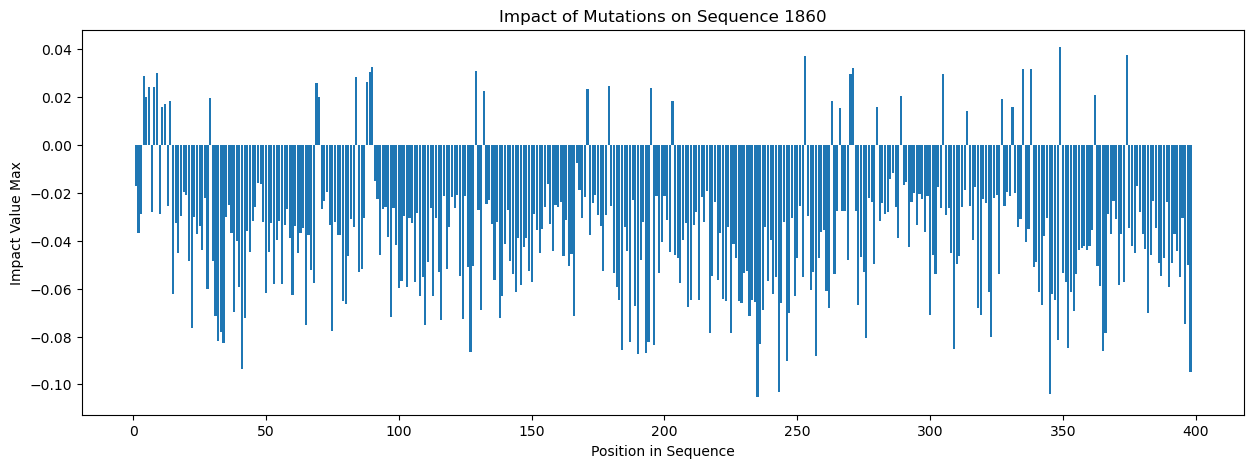
\includegraphics[width=1\linewidth]{5-small_mse_cold_hot.png}
    \caption{Single amino acid mutation effect on sequence 1860}
    \label{fig:seq1860}
  \end{figure}

\begin{figure}
    \centering
    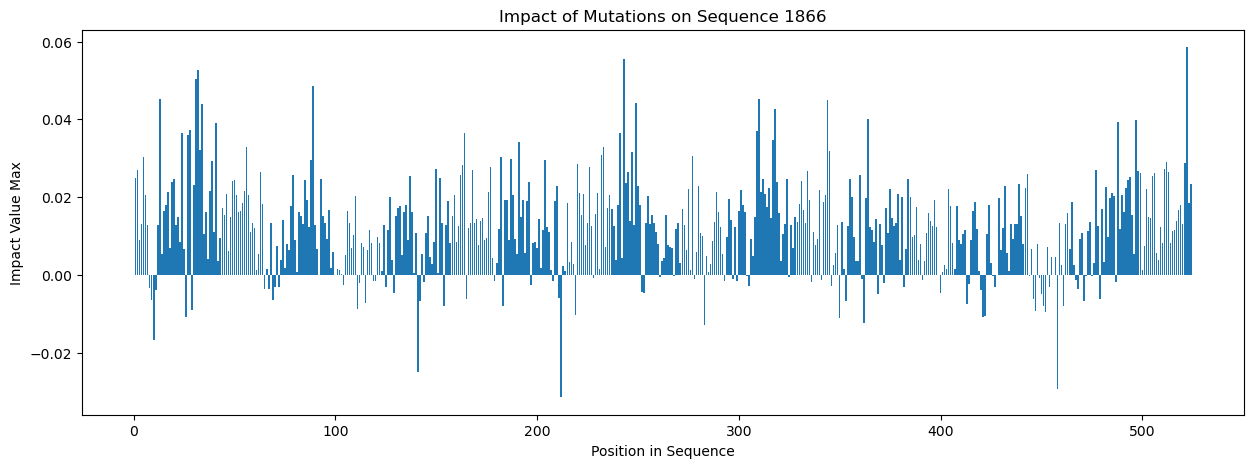
\includegraphics[width=1\linewidth]{5-high_mse_cold_hot.png}
    \caption{Single amino acid mutation effect on sequence 1041}
    \label{fig:seq1866}
  \end{figure}

Two main observations emerge from our experiment. First, the variation across all amino acid mutations is relatively consistent, with changes generally capped at a maximum of 0.10, which corresponds to a variation of up to 20\%. The second observation is that these variations can be both positive and negative, without a clear pattern emerging. These points are crucial as they offer insights into the model's operational dynamics.

Considering the role of specific amino acids in enzyme activity, it's known that only a limited number of amino acids within an enzyme are essential for facilitating a reaction, as explain in Section \ref{section:enzyme}. This implies that the presence or absence of these critical amino acids significantly influences the Michaelis constant, reflecting the enzyme's affinity for a substrate. Ideally, if an enzyme lacks these critical amino acids, the reaction would be severely impaired, leading to a substantially higher Michaelis constant. However, our data indicate that mutations result in values that remain close to the original predictions, suggesting that the model fails to capture the intricate interactions between the protein and the substrate accurately.
  
Enzymes are highly specific, and thus, it would be reasonable to expect that most mutated sequences would result in a higher Michaelis constant (indicating reduced affinity), with only a few exceptions potentially showing a lower constant (suggesting increased affinity). Such cases would be of great interest for enzyme engineering. Yet, the distribution of our results, featuring both positive and negative variations, does not align with this expectation, further highlighting the model's limitations in accurately modeling enzyme-substrate interactions.
  
To further investigate the model's performance, we next examine the distribution of substrates.

\subsection{Substrate Distribution Analysis}

Moving forward from the investigation into protein impacts, which revealed minimal influence on model predictions due to the model's inability to accurately predict the interaction between mutant proteins and substrates, our focus shifts towards the second input: the substrate. This section delves into what we call the substrate distribution, essentially examining the distribution of the Michaelis constant in relation to the different substrates.

Our initial step was to discern how the substrate distribution associated with high prediction errors contrasts with the overall distribution of substrates. Put simply, we aimed to understand how the Michaelis constant is distributed for substrates where the predicted values significantly deviate from their actual values, and to compare this with the broader dataset distribution.

\begin{figure}
    \centering
    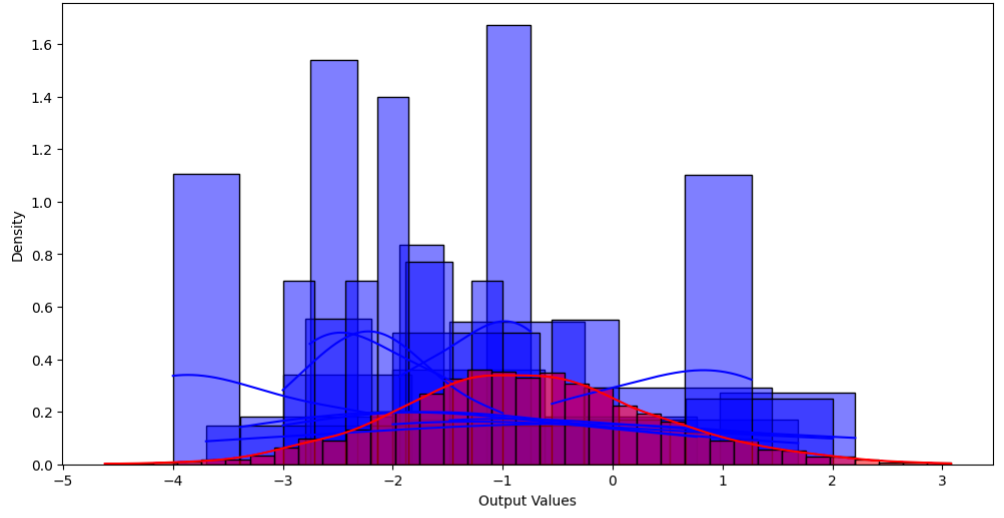
\includegraphics[width=\linewidth]{5-substrate-dist.png}
    \caption{Distribution of substrates with high prediction error}
    \label{fig:substratedist}
\end{figure}

In Figure \ref{fig:substratedist}, the distribution of the 10 substrates exhibiting the highest mean squared error (MSE) is depicted in blue, while the overall substrate distribution is shown in red. Despite the high error rates associated with these 10 substrates, their distribution aligns with the global substrate distribution. This observation suggests that the inaccuracies in predicting the Michaelis constant are not attributable to an atypical distribution of substrates, as the high errors do not correlate with distributions that deviate significantly from the global substrate distribution.

Further analysis of the ProSmith model's results reveals that the most substantial errors arise either from protein-substrate pairs not included in the training set (cold proteins and substrates) — as reflected by the high MSE for this subgroup — or from substrates and proteins that, despite being part of the training set, have Michaelis constants markedly divergent from the distribution specific to these substrates. This insight underscores the challenges the model faces in generalizing predictions across varying conditions, highlighting areas for potential improvement in its predictive accuracy and robustness.

\begin{figure}
    \centering
    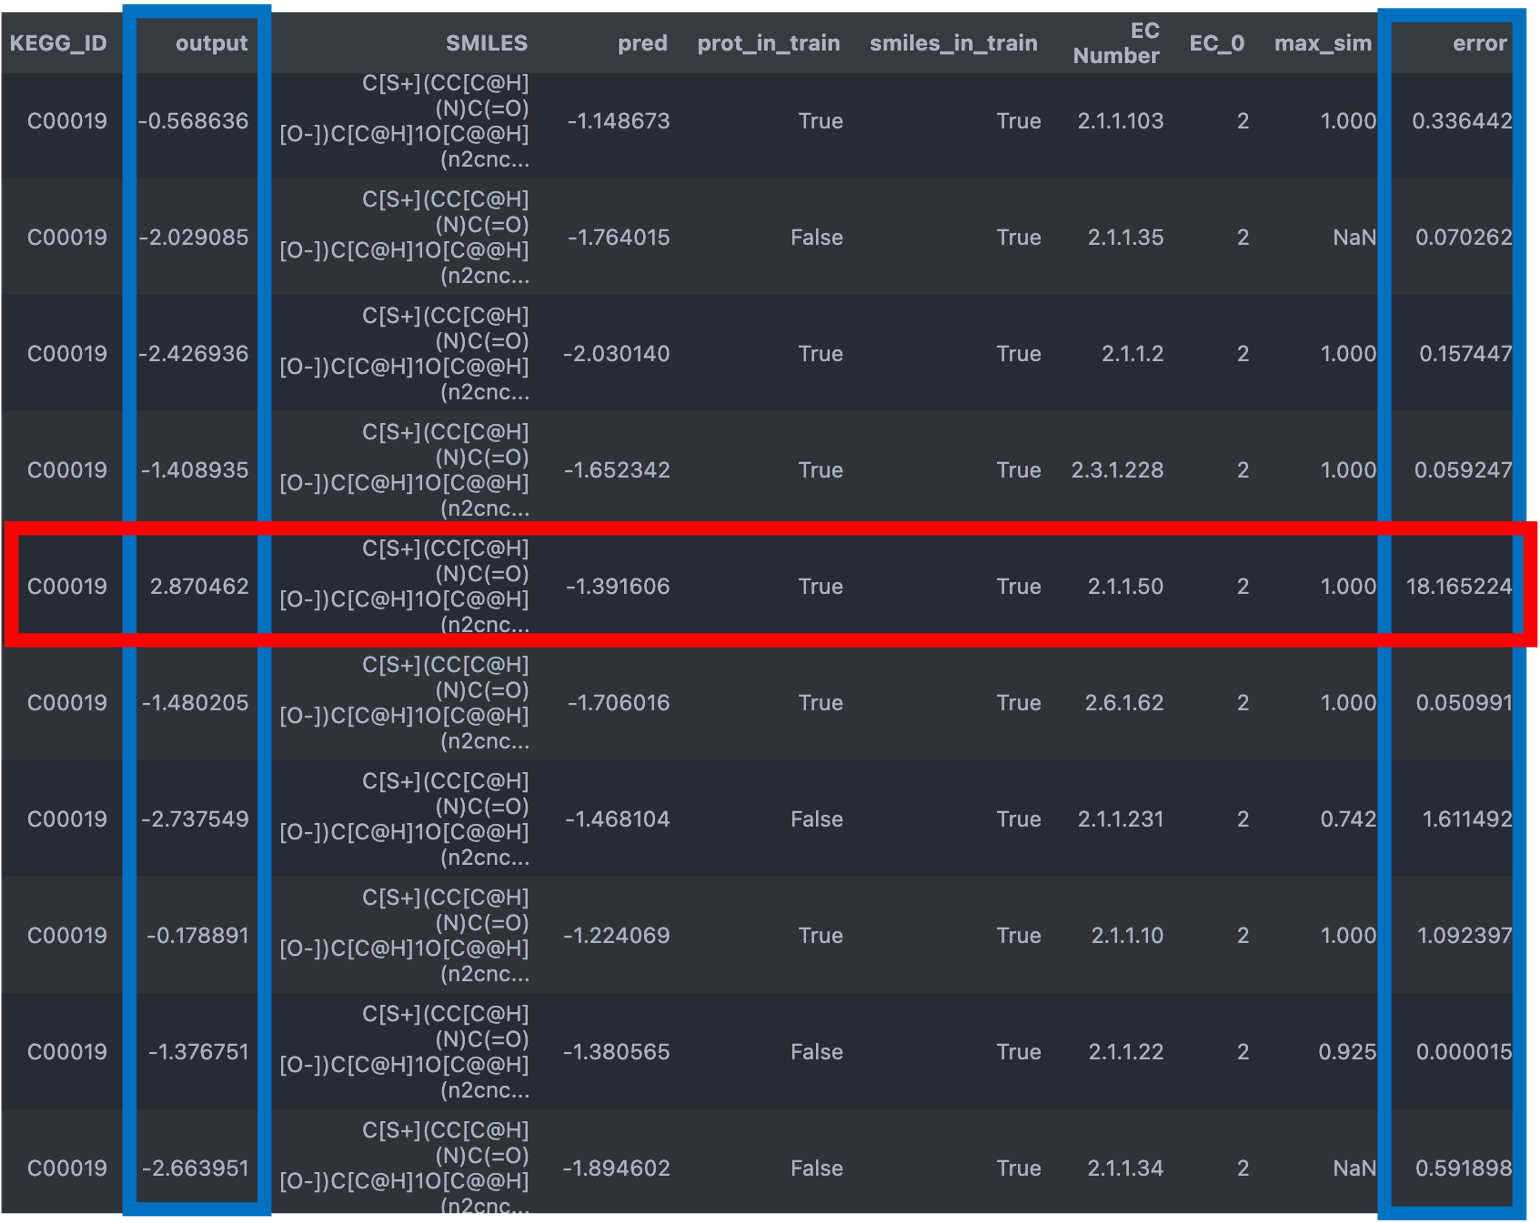
\includegraphics[width=1\linewidth]{5-results1.png}
    \caption{Results for the substrate S-Adenosylmethionine}
    \label{fig:sub1}
  \end{figure}

\begin{figure}
    \centering
    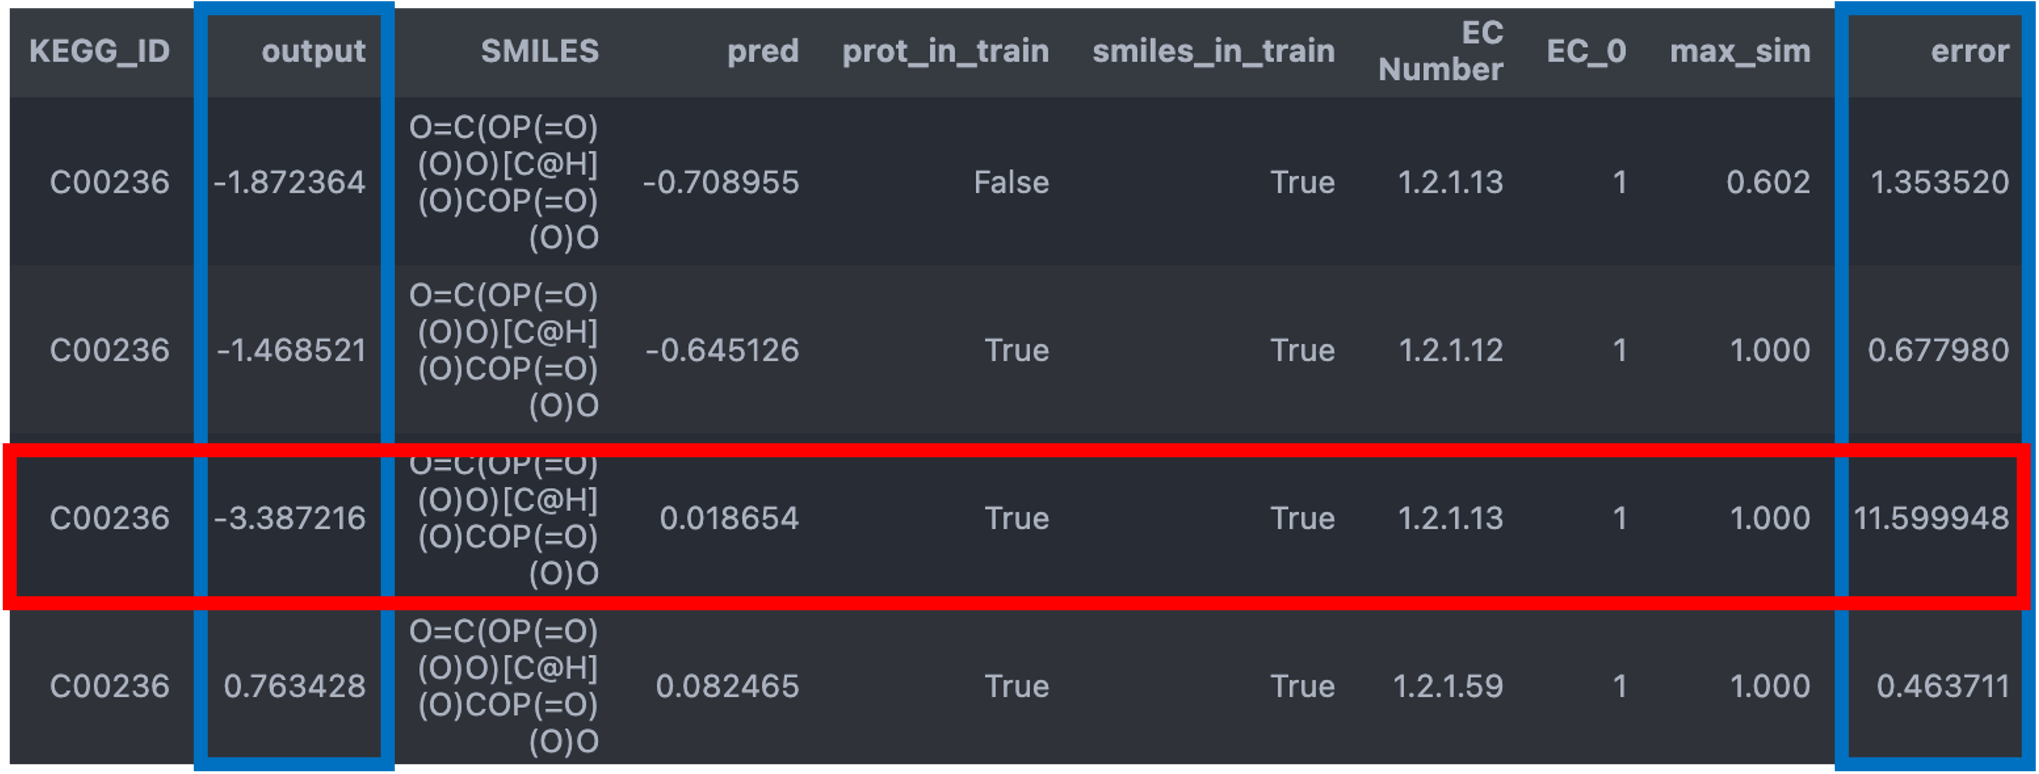
\includegraphics[width=1\linewidth]{5-results2.png}
    \caption{Results for the substrate Succinate semialdehyde}
    \label{fig:sub2}
  \end{figure}

Figures \ref{fig:sub1} and \ref{fig:sub2} examplify this discovery. As it is shown in red, we observe that for the same substrate, when the real Michaelis constant is outside of the general distribution of the substrate, the model is incapable of predicting this value properly and predicts instead a value inside the distribution of this substrate, showing the incapability of the model to predict properly the interaction between the enzyme and its substrate. However, this is a consequent problem as each substrate interact very differently between different enzymes and this element is essential to take into account, which is something ProSmith is incapable of doing.

\subsection{Analaysis Conclusions}

The detailed examination of single amino acid mutation effects reveals that the predicted Michaelis constant fluctuates within a narrow margin, disregarding the fundamental biological principle that an enzyme's specificity is compromised by mutations across its amino acid sequence. This observation signals ProSmith's inadequacy in capturing the essence of enzyme-substrate interactions.

Moreover, the analysis of substrate distribution further elucidates that the most pronounced prediction errors do not stem from substrates with atypical distributions. Instead, they arise from substrates with typical distributions that include some enzymes with markedly distinct Michaelis constants. This finding suggests that ProSmith's predictions are overly reliant on general substrate distribution patterns and lack the sophistication needed to model individual protein-substrate interactions accurately.

Despite ProSmith exhibiting superior performance metrics, such as MSE and coefficient of determination, the model demonstrates a clear deficiency in its ability to predict enzyme-substrate interactions precisely, indicating ample room for improvement. This limitation is particularly evident in its poor coefficient of determination of 0.082 for cold proteins and substrates, highlighting a significant challenge in generalization.

In subsequent chapters, our objective is to explore alternative methods to address these issues. Our aim is to enhance the model's capacity for accurate prediction and generalization across diverse enzyme-substrate interactions, thereby overcoming the limitations observed in ProSmith's current implementation.
